% !TEX TS-program = pdflatex
% !TEX encoding = UTF-8 Unicode

% This is a simple template for a LaTeX document using the "article" class.
% See "book", "report", "letter" for other types of document.

\documentclass[11pt]{article} % use larger type; default would be 10pt

\usepackage[utf8]{inputenc} % set input encoding (not needed with XeLaTeX)

%%% Examples of Article customizations
% These packages are optional, depending whether you want the features they provide.
% See the LaTeX Companion or other references for full information.

%%% PAGE DIMENSIONS
\usepackage{geometry} % to change the page dimensions
\geometry{a4paper} % or letterpaper (US) or a5paper or....
% \geometry{margin=2in} % for example, change the margins to 2 inches all round
% \geometry{landscape} % set up the page for landscape
%   read geometry.pdf for detailed page layout information

\usepackage{graphicx} % support the \includegraphics command and options

% \usepackage[parfill]{parskip} % Activate to begin paragraphs with an empty line rather than an indent

%%% PACKAGES
\usepackage{booktabs} % for much better looking tables
\usepackage{array} % for better arrays (eg matrices) in maths
\usepackage{paralist} % very flexible & customisable lists (eg. enumerate/itemize, etc.)
\usepackage{verbatim} % adds environment for commenting out blocks of text & for better verbatim
\usepackage{subfig} % make it possible to include more than one captioned figure/table in a single float
% These packages are all incorporated in the memoir class to one degree or another...

%%% HEADERS & FOOTERS
\usepackage{fancyhdr} % This should be set AFTER setting up the page geometry
\pagestyle{fancy} % options: empty , plain , fancy
\renewcommand{\headrulewidth}{0pt} % customise the layout...
\lhead{}\chead{}\rhead{}
\lfoot{}\cfoot{\thepage}\rfoot{}

%%% SECTION TITLE APPEARANCE
\usepackage{sectsty}
\allsectionsfont{\sffamily\mdseries\upshape} % (See the fntguide.pdf for font help)
% (This matches ConTeXt defaults)

%%% ToC (table of contents) APPEARANCE
\usepackage[nottoc,notlof,notlot]{tocbibind} % Put the bibliography in the ToC
\usepackage[titles,subfigure]{tocloft} % Alter the style of the Table of Contents
\renewcommand{\cftsecfont}{\rmfamily\mdseries\upshape}
\renewcommand{\cftsecpagefont}{\rmfamily\mdseries\upshape} % No bold!
\usepackage[obeyspaces]{url}

%%% END Article customizations

%%% The "real" document content comes below...

\title{Rossignol user manual}
%\author{Olivier Pisano}
%\date{} % Activate to display a given date or no date (if empty),
         % otherwise the current date is printed 

\begin{document}

\maketitle
\begin{figure}[h!]
\centering

\includegraphics{img/rossignol.png}
\end{figure}
\newpage
\section{Introduction}
\subsection{What is Rossignol?}

Rossignol is a free Web syndication client. Web syndication 
is a mecanism used by a Web site to provide to provide to people with a 
summary of the website recently added content.Rossignol lets the user subscribe 
to syndication feeds and check them for updates. 

Syndication allows users to avoid manually visiting all the websites they are 
interrested in, and presents any new content in a summarized and organized way. 
Rossignol is free software, published under the GNU General Public License. It 
means Rossignol source code can be studied, adapted and modified and the 
resulting software can be distributed under the same license. Therefore 
Rossignol users can insure it respects their liberty. 

\subsection{What does Rossignol mean?}

Rossignol is the french word for nightingale, a small passerine bird commonly 
found in Europe and Asia. Rossignol is pronounced "ROSS - IN - YOL". The name 
was chosen because Rossignol creator is French and the first three consonant
letters are RSS, a format of web syndication. 

\subsection{Key features}
\begin{description}
\item [Feed formats] RSS 1.x, RSS 2.x, Atom.
\item [Supported encoding] UTF-8, all ISO encodings from ISO-8859-1 to
ISO-8859-16.
\item Mozilla Firefox compatibility. 
\item [Supported Operating System] Microsoft Windows,Linux. 

\end{description}

\section{Version notes}
\subsection{What's new in version 0.2?}
\begin{itemize}
\item First Linux version (Ubuntu package)
\item Added documentation (this manual)
\item Added two commands for history handling (in the History menu)
\item Added article description as tooltip in the articles table
\item Added FireFox integration 
\item Now forbids running multiple instances of Rossignol for a given user 
\item Fixed translation of HTML entities
\end{itemize}

\section{Using Rossignol}
\subsection{Installation}
\subsubsection{Microsoft Windows}
To install Rossignol on Microsoft Windows, simply double-click the 
\texttt{install.exe}
file and follow the on-screen wizard. This requires you have administrator 
credentials on the machine you are using. 

\subsubsection{Ubuntu}
To install Rossignol on Ubuntu Linux, double-click the rossignol.deb package 
we provide. This requires your account can sudo on the computer you are using. 
Or you can login as root and type \texttt{dpkg -i rossignol.deb} in the terminal. 
\\
As it is recommanded by the Filesystem Hierarchy Standard, Rossignol installs 
itself in the \texttt{/opt/Rossignol} directory. 

\subsection{User interface}

\begin{figure}[h]
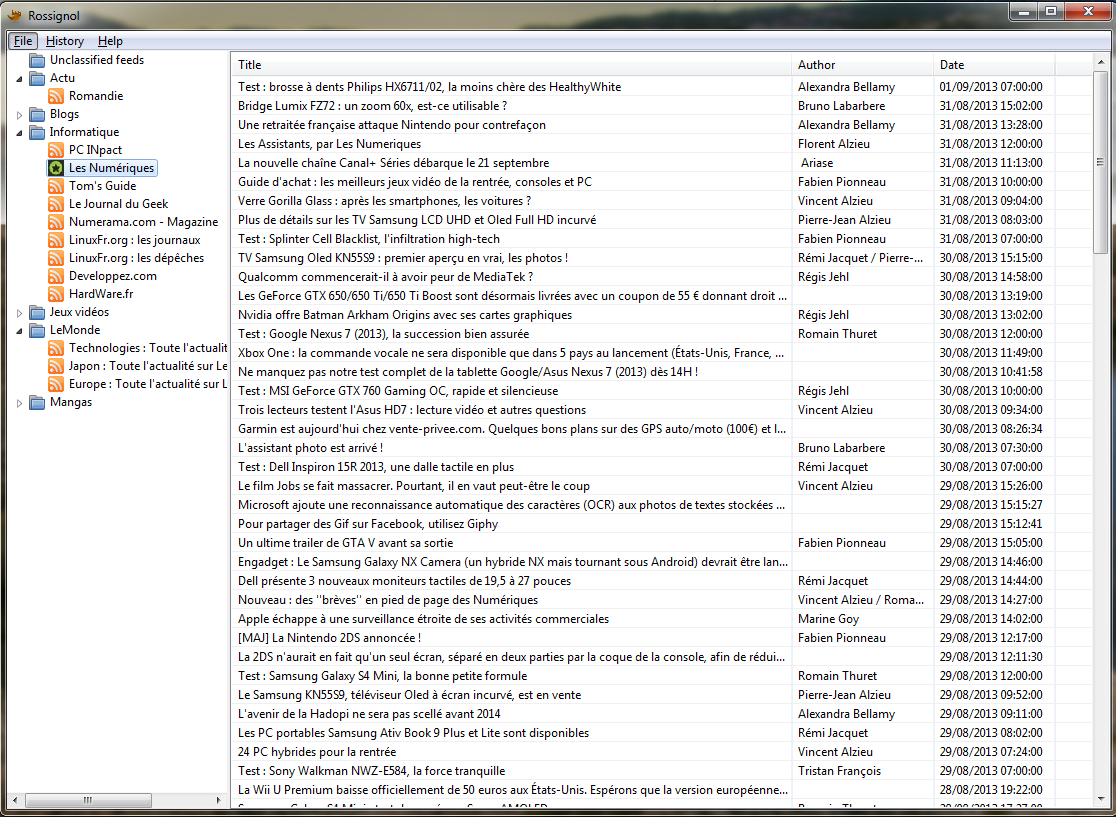
\includegraphics[width=15cm]{img/screen_rossignol.png}
\caption{Rossignol main window}
\end{figure}

Rossignol main window is divided in two parts:
\begin{itemize}
\item On the left is the feed tree. It enables you to organize the feeds 
subscribed. On the first time Rossignol is started, it contains only one empty 
group: the "unclassified feed" group. This group is the default group for 
storing feeds without organizing them and cannot be removed by the user.
\item On the right is the article table. When a feed is selected, it displays 
its content. 
\end{itemize}

\subsubsection{Subscribing to new feeds}

You can add new feeds in Rossignol in two ways. The manual way is to add the 
feed URL (address) by yourself. To do that you can use the "New feed..." 
command from the File menu. It will display a popup dialog entitled 
"Add new feed...".

\begin{figure}[h]
\centering
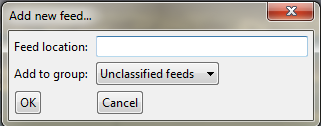
\includegraphics{img/add_feed_dialog.png}
\caption{Add feed dialog}
\end{figure}

Simply copy/paste the feed address from your browser to the "Feed location" 
text field and click on the OK button to subscribe to it.

Firefox users can add a feed in Rossignol directly from their browser. 
When displaying a feed in Firefox, in the "subscribe to this feed using" menu, 
select "Choose an application" and browse your filesystem to choose the 
Rossignol executable. Click on the "subscribe now" button to send the feed data 
from Firefox to Rossignol. 

\subsubsection{Organizing your feeds}

By default, the only group in the feeds tree is the "Unclassified feeds" group. 
It is good for having a few feeds in it, but as soon as you'll get more and more
feeds, you'll need a way to organize them properly.

You can create new groups in the feed tree by selecting the "New group" command 
from the File menu. This creates a new group in the tree and asks you to name 
it. You can rename a group (including the "Unclassified feeds" one) by 
right-clicking it and selecting the rename command. 

You can move a feed from one group to another by drag\&drop'ing it on a group 
icon. 

To unsubscribe from a feed, right-click it and select the "Remove" command. You
can also unsubscribe from a whole group at once the same way. 

\subsubsection{History handling}

As time goes on, Rossignol archives every article on your disk. If you want to 
clean up and retrieve some disk space, you can use commands from the History 
menu.

The "Remove old articles..." command removes articles older than a certain limit 
you can specify. It diplays a dialog where you can choose the period of time 
to keep from you history. Any article older than this period will be removed 
from your feeds. 

\begin{figure}[h]
\centering
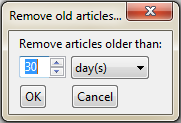
\includegraphics{img/remove_old_articles_dialog.png}
\caption{The remove old articles dialog}
\end{figure}


The "Remove feed history" destroys all the history kept on the disk. Only the 
articles still present in the original feed on the internet will be kept. 

\section{User-specific files}

Now that you know Rossignol keeps files for you on the disk, you are probably 
curious where these files are. 
\begin{itemize}
\item On Microsoft Windows, Rossignol follows Microsoft recommandations and 
stores them in \path{%APPDATA%\Rossignol}. The actual folder identified by the 
\path environment variable depends on your Windows version and your 
operating system language. Starting from Windows Vista, it is 
\path{C:\users\username\AppData\Roaming}.
\item On Linux, Rossignol follows the FreeDesktop.org guidelines and stores 
files in \path{~/.config/Rossignol}. As usual, the tilde character refers
to the user home directory (usually \path{/home/username} on Linux).
\end{itemize}


\end{document}
